%%% Laboratory	 Notes
%%% Template by Mikhail Klassen, April 2013
%%% Contributions from Sarah Mount, May 2014
%%% Updated by Muhammad Davi, September 2022
\documentclass[a4paper]{tufte-handout}
\usepackage{lab_notes}

\title{Practice Big Data}
\date{2022}

\begin{document}
\maketitle

%%%%%%%%%%%%%%%%%%%%%%%%%%%%%%%%%%%%%%%%%%%%%%%%%%%%%%%%

\begin{projects}
	\begin{description}
		\item [Muhammad Davi, S.Kom., M.Cs.] sebagai dosen pengampu matakuliah practice big data\footnote{Dosen Prodi Teknologi Rekayasa Komputer Jaringan, Jurusan Teknologi Informasi dan Komputer, Politeknik Negeri Lhokseumawe}.
		\item [Peserta dan Kelompok] matakuliah practice big data adalah sebegai berikut:

\begin{table}[!ht]
\caption{Peserta dan Kelompok Matakuliah Practice Big Bata}
\label{tab:peserta}
\centering
\begin{tabular}{llr} 
\toprule
NIM 	&	Nama &	Akun Github\\
\midrule
Kelompok 1\\
\midrule
1 gram &	472,764,897 &	\url{https://github.com/snim2/Terminus} \\
2 gram &	6,626,604,215 &	65.6\\
3 gram &	23,260,642,968 &	218.1\\
4 gram &	32,262,967,656 &	293.5\\
5 gram &	24,492,478,978 &	221.5\\
\midrule
Kelompok 2\\
\midrule
1 gram &	261,823,186 &	2.6\\
2 gram &	3,383,379,445 &	32.1\\
3 gram &	10,565,828,499 &	94.8\\
4 gram &	12,987,703,773 &	113.1\\
\midrule
Kelompok 3\\
\midrule
1 gram &	291,639,822 &	3\\
2 gram &	3,923,370,881 &	38.3\\
3 gram &	12,368,376,963 &	113.9\\
4 gram &	15,118,570,841 &	135\\
\midrule
Kelompok 4\\
\midrule
1 gram &	188,660,459 &	1.9\\
2 gram &	2,000,106,933 &	19.1\\
3 gram &	5,186,054,851 &	46.8\\
4 gram &	5,325,077,699 &	46.6\\
\midrule
Kelompok 5\\
\midrule
1 gram	&	191,545,012	&	2\\
2 gram	&	2,516,249,717	&	24.3\\
3 gram	&	7,444,565,856	&	68\\
4 gram	&	8,913,702,898	&	79.1\\
\midrule
\end{tabular}
\end{table}
	\end{description}
\end{projects}

%%%%%%%%%%%%%%%%%%%%%%%%%%%%%%%%%%%%%%%%%%%%%%%%%%%%%%%%

\begin{maybe}
    \begin{itemize}
    	\item Matakuliah Practice Big Data
    	\begin{itemize}
    	\item Waktu: 13.30 - 16.00, 16.20 - 18.00\footnote{Istirahat dan Sholat Ashar 20 Menit}
    	\item Ruang: Lab 3\footnote{Lab Jaringan dan Multimedia di Lantai Dasar Gedung Utama}
    	\item Penilaian\footnote{Sesuai ketenuan dari Kepala Lab}
    	\begin{itemize}
    	\item Responsi Kompetensi
    	\item Sikap
    	\item Laporan
    	\item Seminar
    	\item UAS
    	\item Hasil/Benda kerja
    	\end{itemize}
    	\end{itemize}
    	\item Sebelum masuk lab wajib berbaris dan berdo'a terlebih dahulu.
    	\item Referensi
    	\begin{itemize}
    		\item Buku Ajar Big Data \citep{Mursyidah2020}.
    	\end{itemize}
    \end{itemize}
\end{maybe}

%%%%%%%%%%%%%%%%%%%%%%%%%%%%%%%%%%%%%%%%%%%%%%%%%%%%%%%%
\newpage
\newday{8 September 2022}

\newthought{Introduction \& Preparation} \\
Pada pertemuan pertama, kegiatan lab adalah perkenalan dan persiapan kebutuhan untuk praktik big data. Setelah dosen pengampu memperkenalkan diri dan matakuliah yang diajarkan, dilanjutkan perkenalan dari setiap mahasiswa dah hasilnya dapat dilihat pada Tabel \ref{tab:perkenalan}.

\begin{table}[!ht]
\caption{Hasil Perkenalan Mahasiswa}
\label{tab:perkenalan}
\centering
\begin{tabular}{llr} 
\toprule
Nama 	&	Asal Sekolah 	&	Alamat\\
\midrule
1 gram &	472,764,897 	&	\url{https://github.com/snim2/Terminus} \\
2 gram &	6,626,604,215 	&	65.6\\
3 gram &	23,260,642,968 	&	218.1\\
4 gram &	32,262,967,656 	&	293.5\\
5 gram &	24,492,478,978 	&	221.5\\
\midrule
1 gram &	261,823,186 	&	2.6\\
2 gram &	3,383,379,445 	&	32.1\\
3 gram &	10,565,828,499 	&	94.8\\
4 gram &	12,987,703,773 	&	113.1\\
\midrule
1 gram &	291,639,822 	&	3\\
2 gram &	3,923,370,881 	&	38.3\\
3 gram &	12,368,376,963 	&	113.9\\
4 gram &	15,118,570,841 	&	135\\
\midrule
1 gram &	188,660,459 	&	1.9\\
2 gram &	2,000,106,933 	&	19.1\\
3 gram &	5,186,054,851 	&	46.8\\
4 gram &	5,325,077,699 	&	46.6\\
\midrule
1 gram	&	191,545,012		&	2\\
2 gram	&	2,516,249,717	&	24.3\\
3 gram	&	7,444,565,856	&	68\\
4 gram	&	8,913,702,898	&	79.1\\
\midrule
\end{tabular}
\end{table}

Setelah perkenalan, setiap mahasiswa membuat akun github dan akun discord sebagai media komunikasi dan tempat bekerja secara berkelompok. Hasil dari kegiatan tersebut dapat dilihat pada Tabel \ref{tab:peserta} dan Server Discord pada alamat \url{https://discord.gg/V32EWUx6}.

\hrulefill

%%%%%%%%%%%%%%%%%%%%%%%%%%%%%%%%%%%%%%%%%%%%%%%%%%%%%%%%
\newpage
\newday{15 September 2022}

\newthought{Instalasi Apache Hadoop} \\
{\tt http://adsabs.harvard.edu/cgi-bin/bib\_query?1993ApJ...406..528G}

\begin{figure}
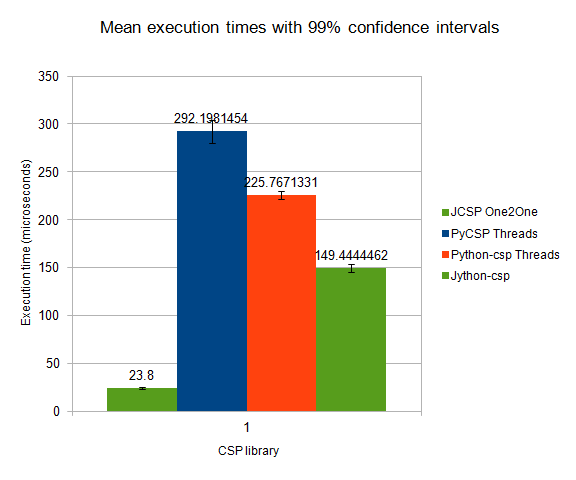
\includegraphics[scale=0.65]{benchmark}
\caption{Gambar 1}
\label{gam:gambar}
\end{figure}


\hrulefill

%%%%%%%%%%%%%%%%%%%%%%%%%%%%%%%%%%%%%%%%%%%%%%%%%%%%%%%%
\newpage
\newday{22 September 2022}
\textit{N.B.: Setiap mahasiswa membuat laporan hasil praktik dengan format yang telah ditentukan. Template laporan dapat di download pada alamat \url{https://github.com/snim2/Terminus}.}

\newthought{Instalasi Apache Pig} \\

\section{Laporan Mahasiswa}
\begin{enumerate}
\item Nama Mahasiswa \\
\textit{isi laporan}
\item Nama Mahasiswa \\
\textit{isi laporan}
\item Nama Mahasiswa \\
\textit{isi laporan}
\end{enumerate}


\hrulefill

%%%%%%%%%%%%%%%%%%%%%%%%%%%%%%%%%%%%%%%%%%%%%%%%%%%%%%%%
\newpage
\bibliographystyle{plain}
\bibliography{lab_notes}

\end{document}

\begin{comment}
\section{Laporan Mahasiswa}
\begin{enumerate}
\item Nama Mahasiswa \\
\textit{isi laporan}
\item Nama Mahasiswa \\
\textit{isi laporan}
\item Nama Mahasiswa \\
\textit{isi laporan}
\end{enumerate}
\end{comment}
